\documentclass[11pt,conference]{IEEEtran}

\usepackage{amsmath,amssymb,amsfonts}
\usepackage{algorithmic}
\usepackage{graphicx}
\usepackage{subcaption}
\usepackage{textcomp}
\usepackage{xcolor}
\usepackage[colorlinks]{hyperref}
\usepackage[style=ieee]{biblatex}
\addbibresource{sources.bib}

\renewcommand{\algorithmiccomment}[1]{\% #1}

\begin{document}

\title{Proposal: Proving Termination of \texttt{zelda-mosaic} Algorithms under Conditions on the Input}

\author{\IEEEauthorblockN{Justin Do}
\IEEEauthorblockA{\textit{Computer Science} \\
\textit{UNC Chapel Hill}\\
Chapel Hill, USA \\
\texttt{justindo@cs.unc.edu}}
\and
\IEEEauthorblockN{D. Ben Knoble}
\IEEEauthorblockA{\textit{Computer Science} \\
\textit{UNC Chapel Hill}\\
Chapel Hill, USA \\
\texttt{david3@cs.unc.edu}}
}

\maketitle

% \begin{abstract}
% \end{abstract}

% \begin{IEEEkeywords}
% \end{IEEEkeywords}

\section{Introduction}

We have previously developed \texttt{zelda-mosaic}~\cite{zelda_mosaic} which
includes MATLAB~\cite{matlab} code to create tiled ``mosaics'' from a set of
smaller input images. We propose now to prove termination of our
mosaic-generation algorithms.

In the original work, we took a series of related images (specifically, from one
of the many ``Legend of Zelda'' ({\copyright} Nintendo) games) and automatically
stitched them together to form mosaics of game-related artwork.
\figurename~\ref{F:zelda-mosaic-sample} showcases an example output. The program
is extendable and has been successfully used on several different sizes of
inputs and for applications beyond the original project.

\begin{figure*}[!t]
    \centering
    \begin{subfigure}{0.35\textwidth}
        
\includegraphics[width=\linewidth]{img/oracleofages-original.jpg}
        \caption{Original key-art}
    \end{subfigure}
    \begin{subfigure}{0.35\textwidth}
        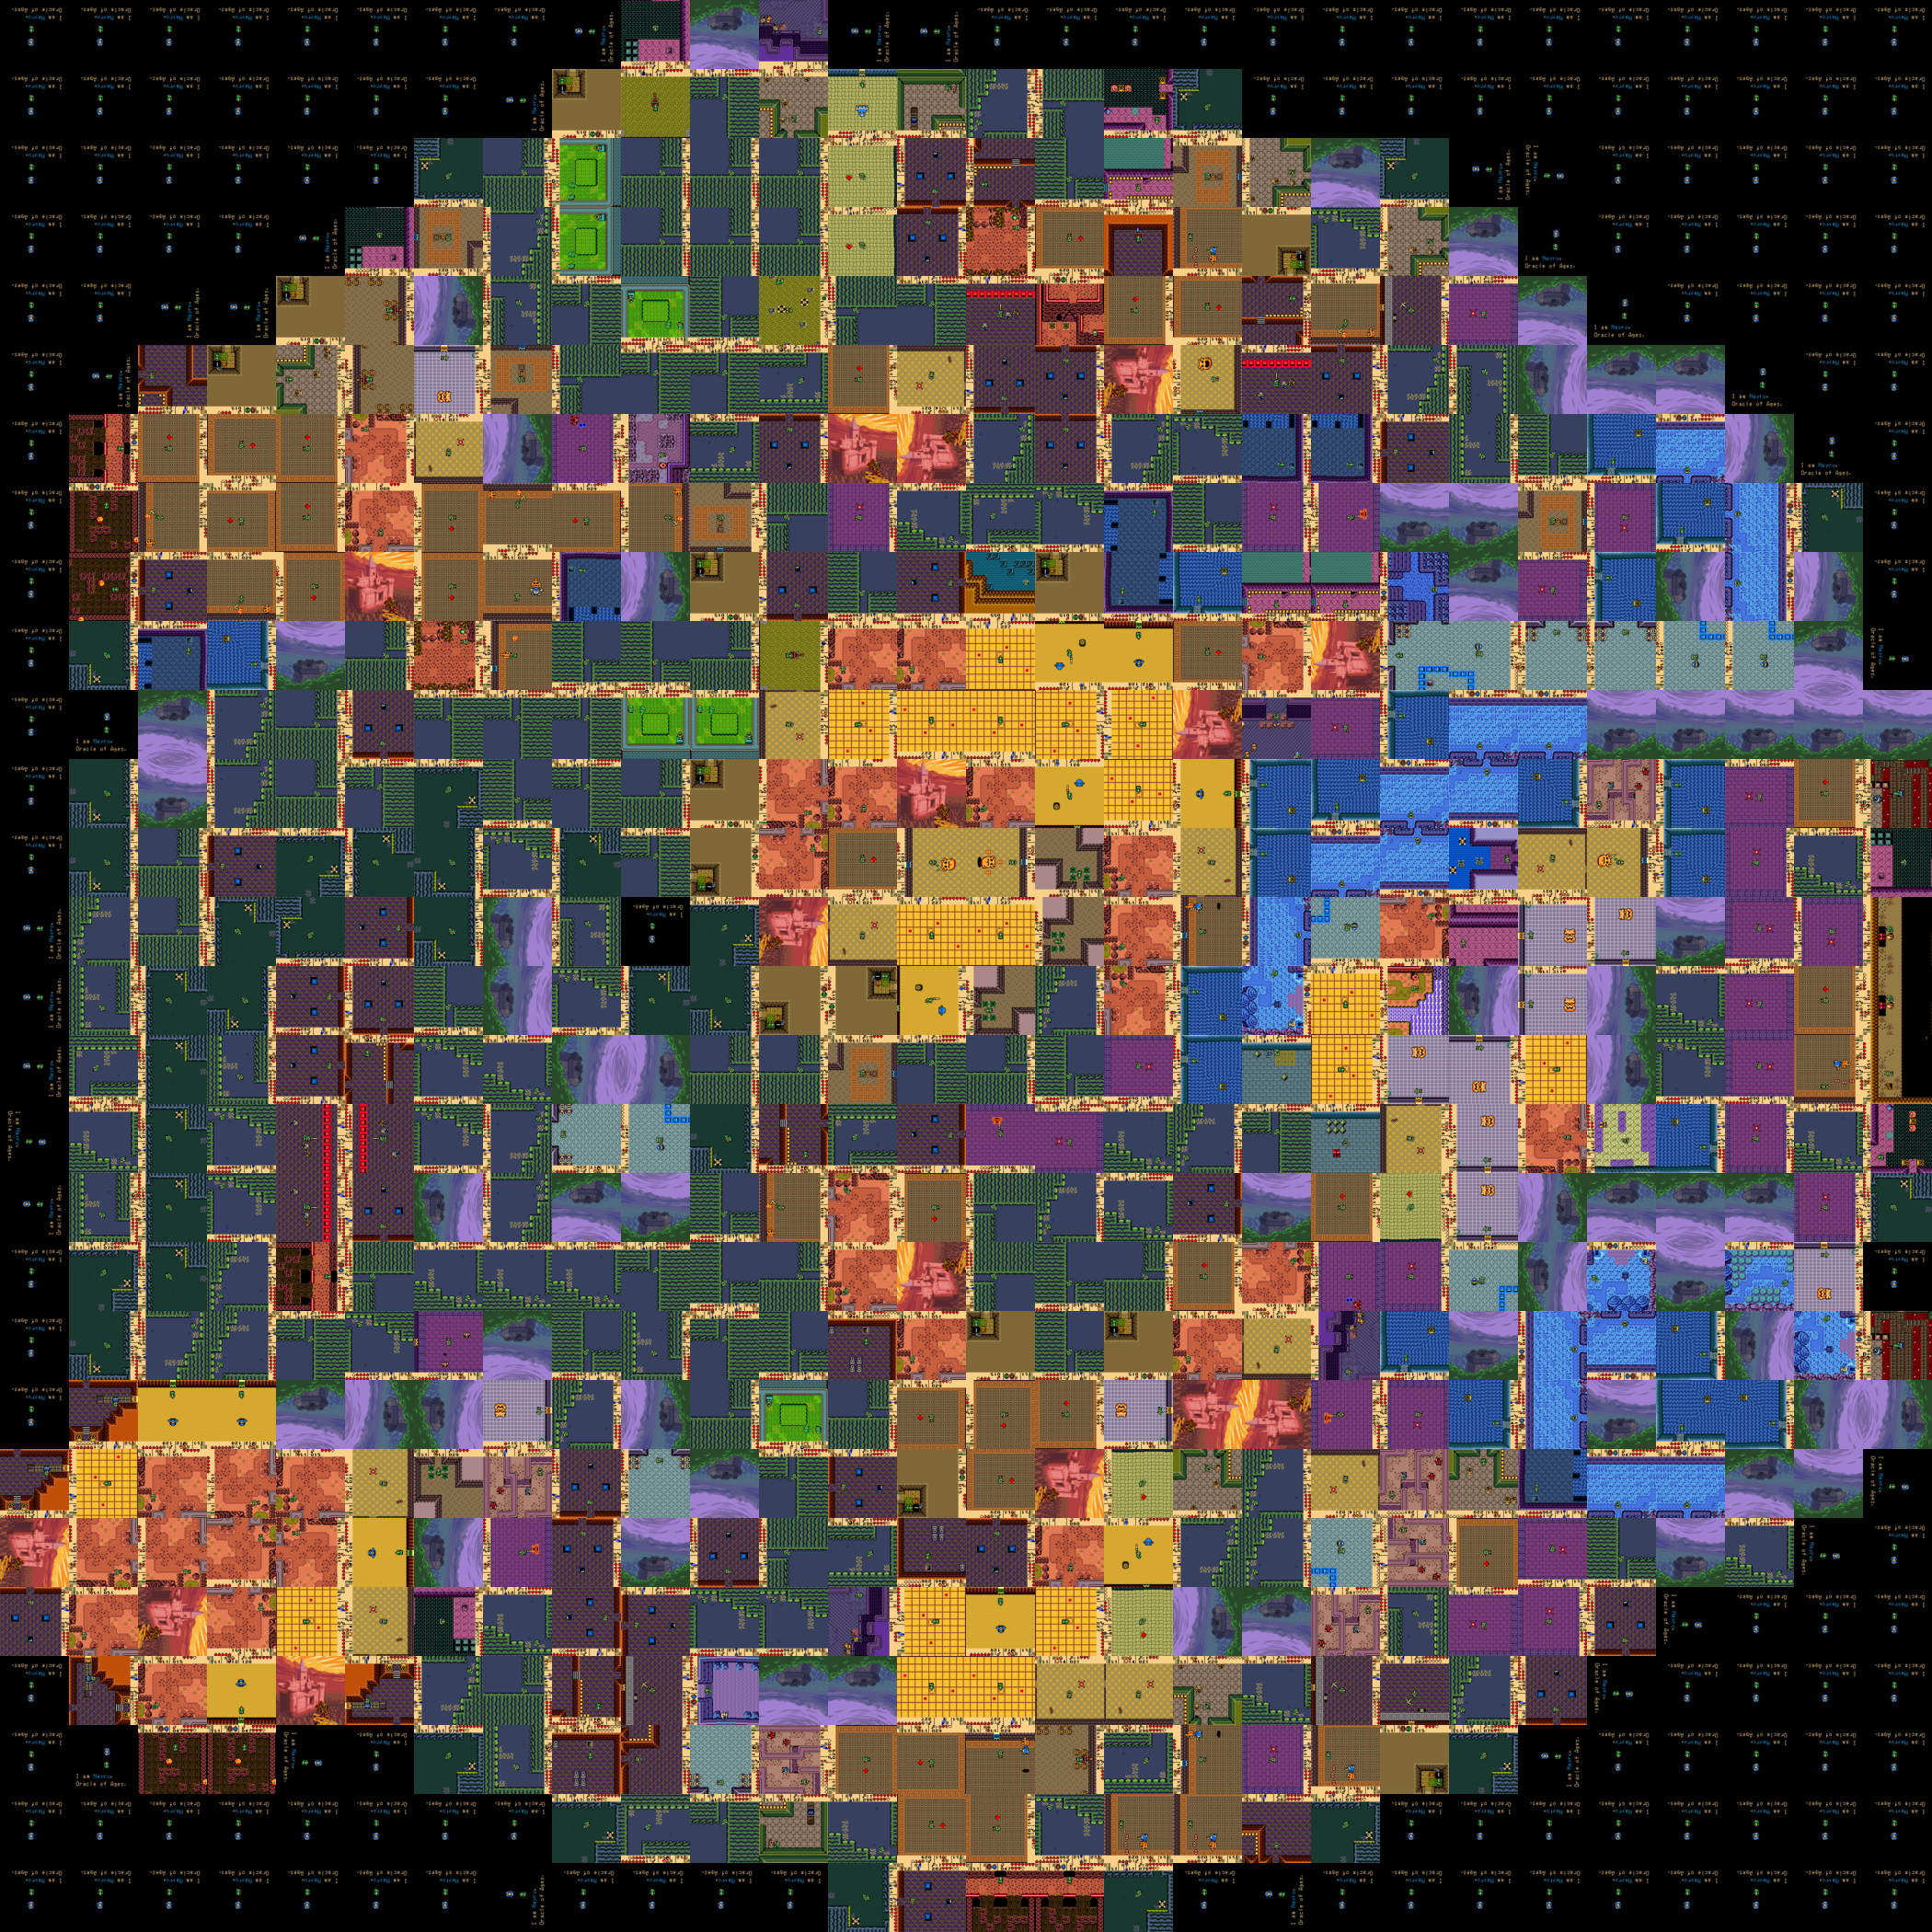
\includegraphics[width=\linewidth]{img/oracle_of_ages_v1.png}
        \caption{Version 1 Mosaic}
    \end{subfigure}
    \begin{subfigure}{0.35\textwidth}
        \includegraphics[width=\linewidth]{img/oracle_of_ages_v2.png}
        \caption{Version 2 Mosaic}
    \end{subfigure}
    \begin{subfigure}{0.35\textwidth}
        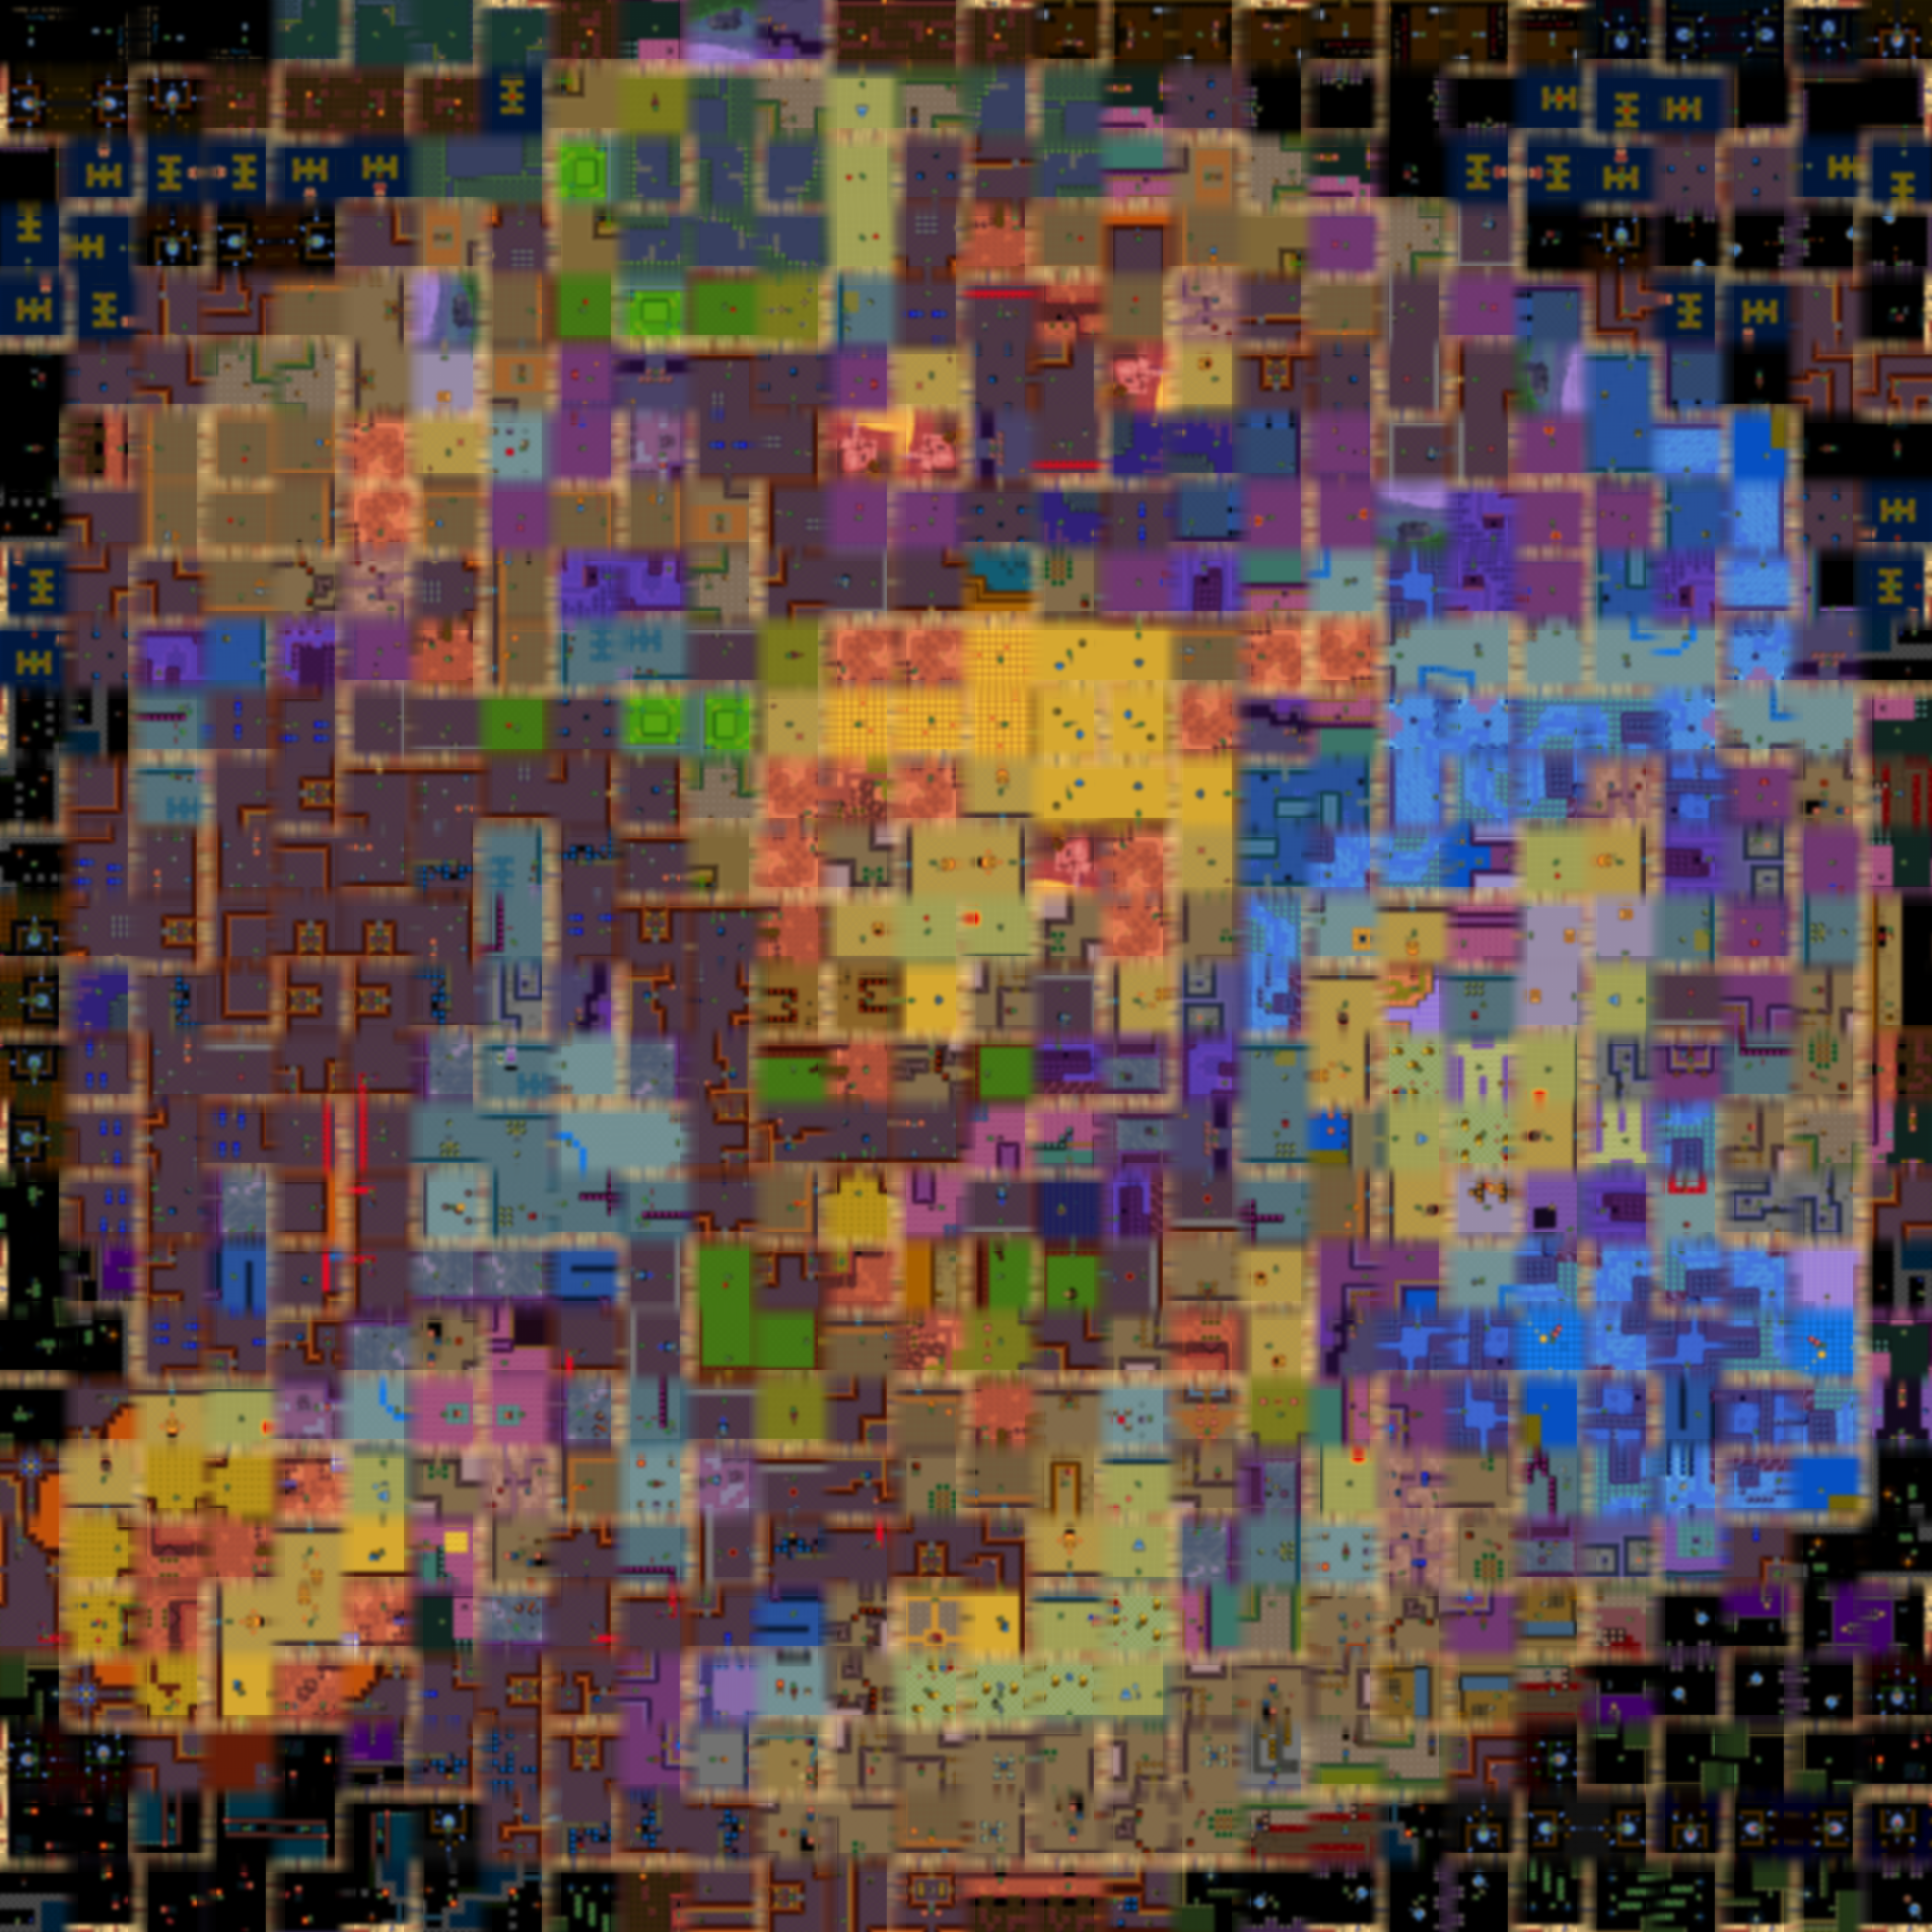
\includegraphics[width=\linewidth]{img/oracle_of_ages_v3.png}
        \caption{Version 3 Mosaic}
    \end{subfigure}
    \begin{subfigure}{0.35\textwidth}
        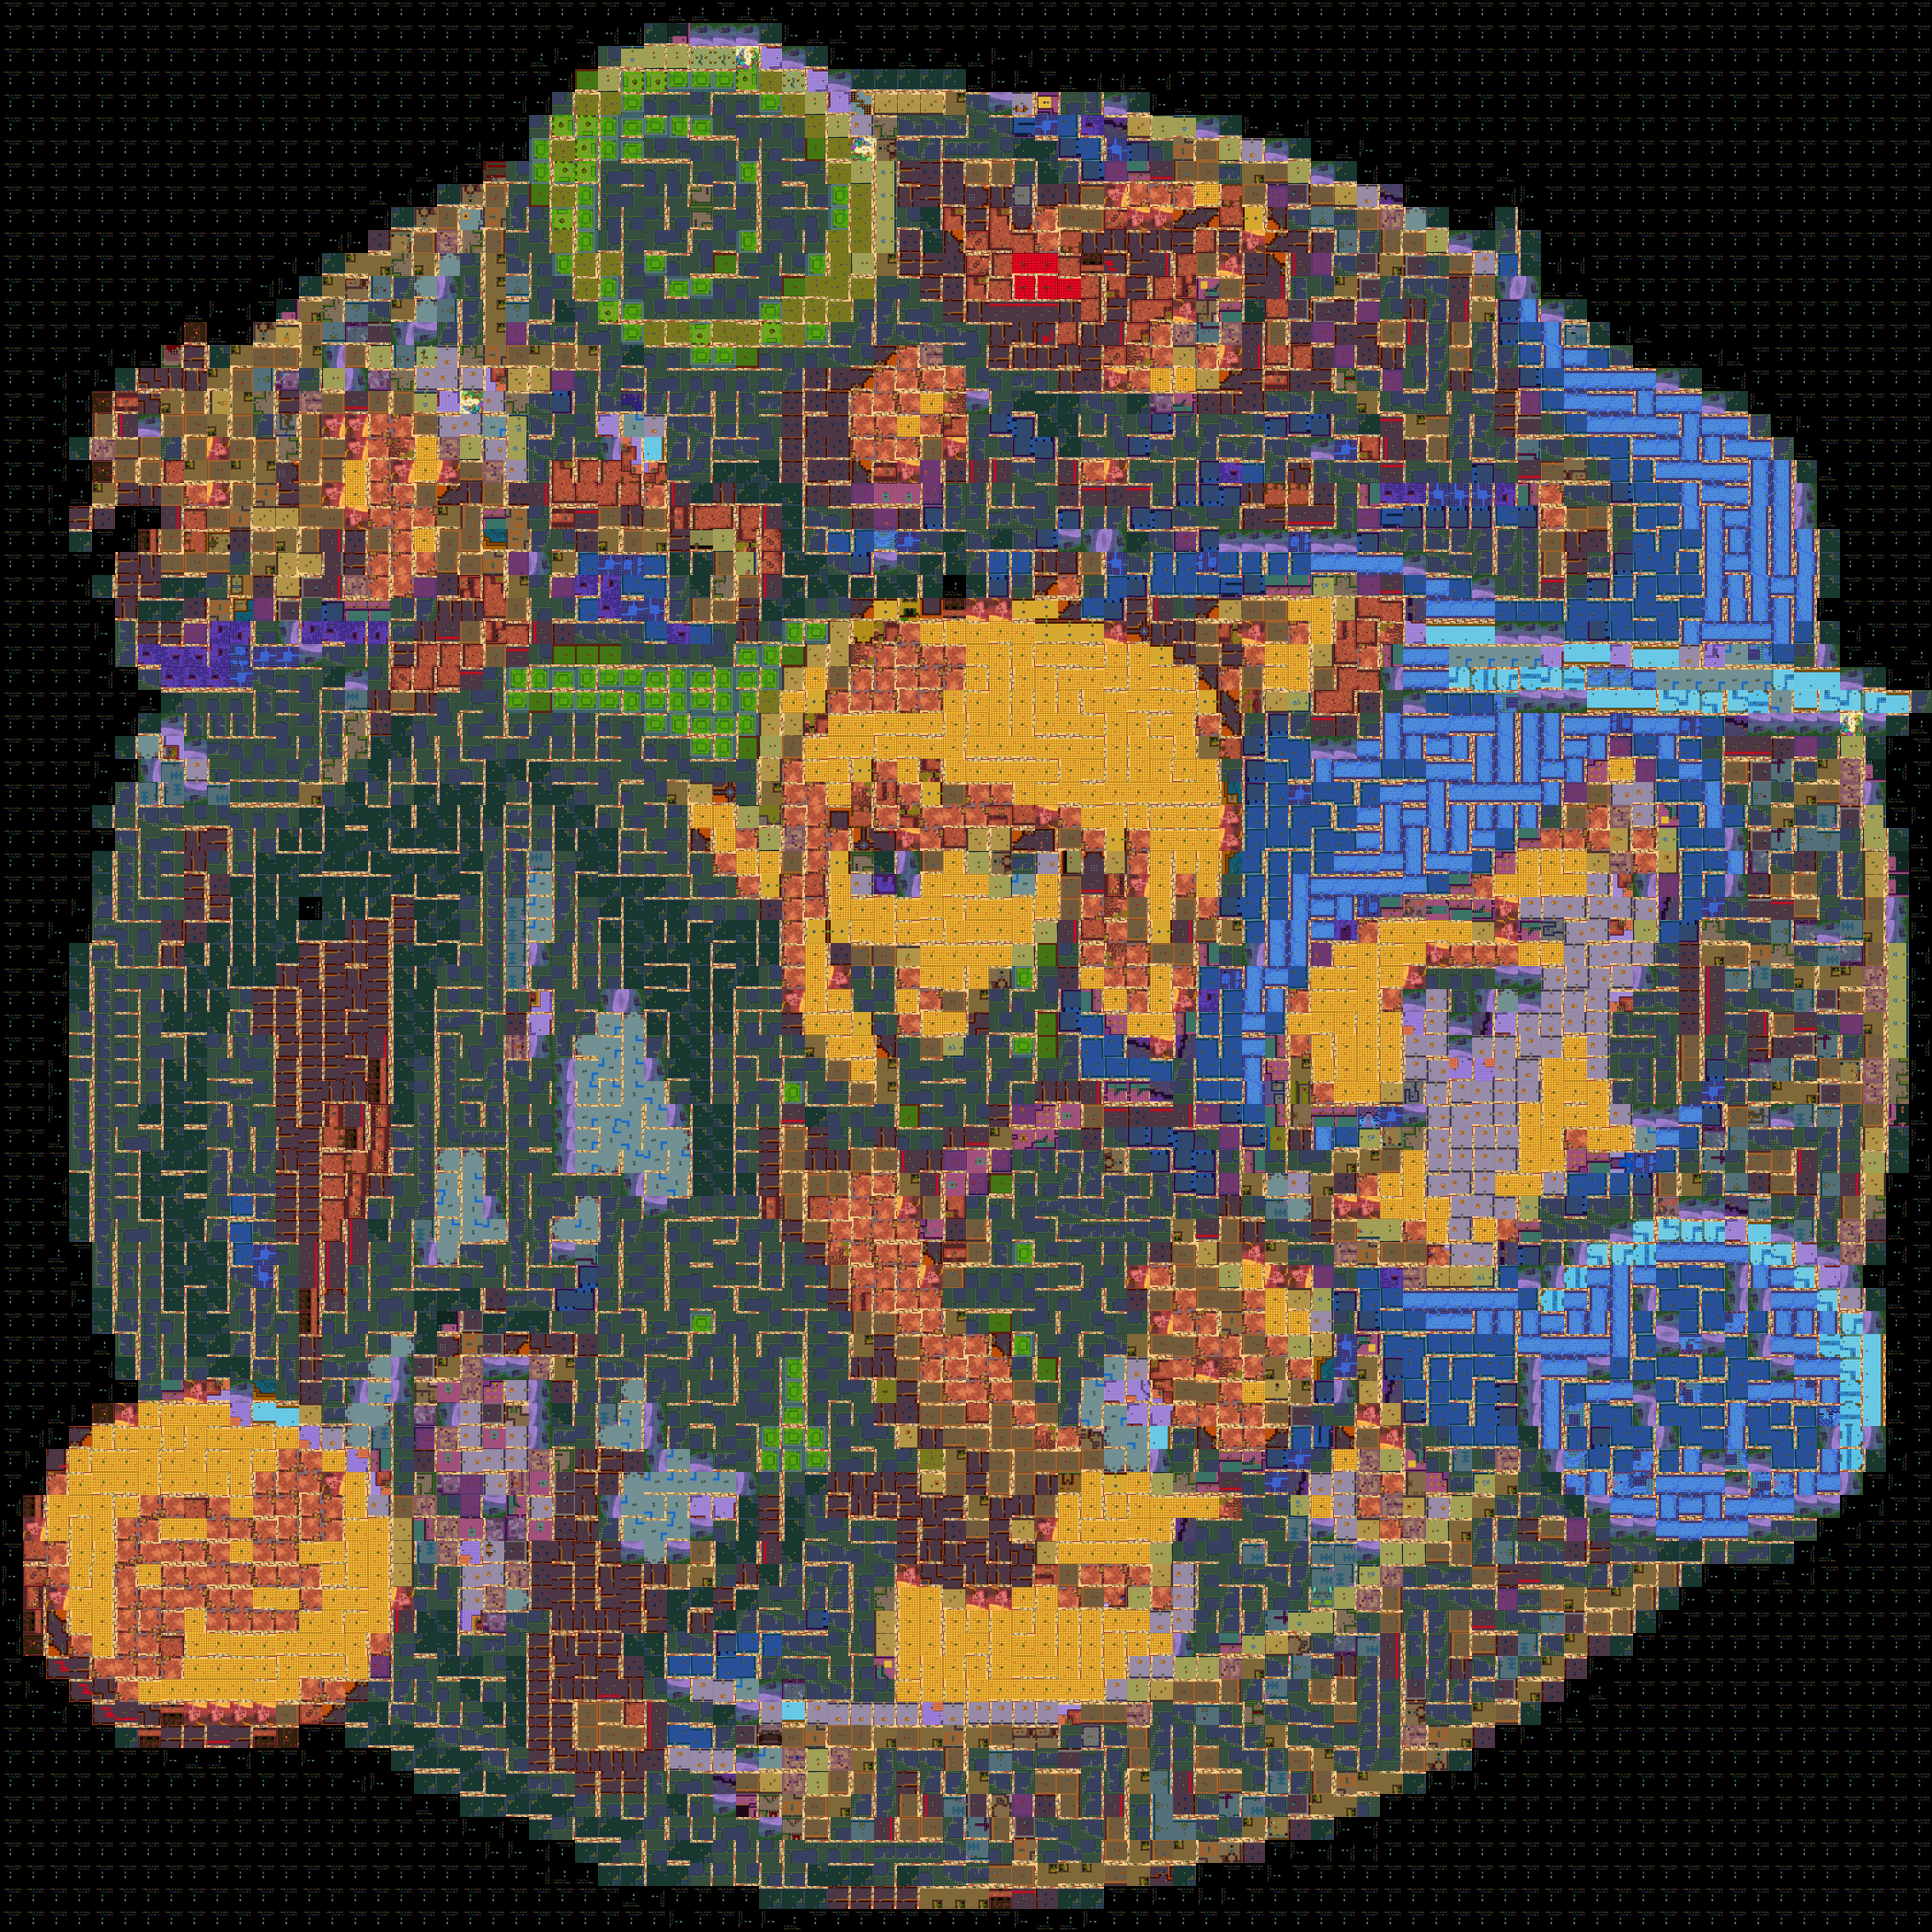
\includegraphics[width=\linewidth]{img/oracle_of_ages_v1_smaller.png}
        \caption{Version 1 Mosaic with smaller inputs}
    \end{subfigure}
    \begin{subfigure}{0.35\textwidth}
        \includegraphics[width=\linewidth]{img/oracle_of_ages_v3_smaller.png}
        \caption{Version 3 Mosaic with smaller inputs}
    \end{subfigure}
    \caption{\texttt{zelda-mosaic} sample}\label{F:zelda-mosaic-sample}
\end{figure*}

We iteratively developed three versions after our initial proof-of-concept. Each
version refines the algorithm of the previous version (for details,
see~\ref{S:AlgDet}). Starting from a working prototype (version
1,~\ref{S:algv1}), we proceeded to add limited duplication (version
2,~\ref{S:algv2}) and seam-blending (version 3,~\ref{S:algv3}). We also further
refined mosaic quality by stitching smaller images, at a performance cost. The
original presentation is publicly available~\cite{zelda_mosaic_pres}, as is a
separate video-recording~\cite{zelda_mosaic_vid}.

Now we propose to examine these algorithms as implemented in the MATLAB source
and prove, if possible, their termination given well-conditioned input. What
necessary conditions are remains to be seen, but likely includes constraints on
the sizes of each individual input image and the size of the key art target
image.

\subsection{Motivation}

There are several factors that motivate our interest in this particular
algorithm, its particular implementation, and its properties.

Personally, it is a project we've already invested in, and one which we enjoy
studying.

Academically, it presents several unique opportunities. First, as far as we can
tell, there have been no studies on either termination-properties of mosaic
algorithms or of MATLAB code. Further, we have found no attempt to formalize
details of the MATLAB programming language\footnote{This may in part be due to
the proprietary, closed-source nature of MATLAB\@. Nevertheless, we hope to make
an attempt, though it must be grounded in the knowledge that any proof can only
hold if indeed the MATLAB environment faithfully implements the semantics it
claims. There are formalizations of a particular MATLAB toolkit known as
Stateflow~\cite{Hamon_2005,Hamon_2007} but none that we have found for general
MATLAB programming.}. Thus already in studying this particularly narrow problem
we have an opportunity to extend the space of studies in formal-methods and
their applications to the programmer and their programs.

Second, we as students of these formal methods lack experience in formalizing
these details about specific algorithms. The Logical Foundations
text~\cite{Pierce:SF1} has proven a great resource in learning about these
principles on small examples, and our study of \texttt{zelda-mosaic} will make
an excellent opportunity to extend our practical knowledge of the field.

Lastly, termination and its decidability has always been a study of interest to
the logician, the mathematician, and the computer scientist. From Hilbert's
\textit{Entscheidungsproblem} to Turing's Halting problem~\cite{Cook_2011}, the
world of algorithms is generally concerned with what is, indeed, computable.
While we make no attempt here to prove termination of arbitrary or even
restricted MATLAB programs (likely a Sisyphean task), we can at least attempt to
push the boundaries of the undecidable Halting problem for this specific
program.

\section{Algorithm Details}\label{S:AlgDet}

In this section, we present the high-level details of the three algorithms about
which we aim to prove termination. We begin with a brief overview of the
relevant inputs before proceeding to give pseudo MATLAB-code for each version of
the algorithm accompanied by textual explanation.

\subsection{Background}

Across each of the three versions, the inputs are the same. The three inputs are

\begin{enumerate}
    \item an image \textit{key art}, the target image the final mosaic will
        replicate
    \item a series of \textit{thumbnails}, smaller images which will form the
        tiles of the mosaic
    \item an integer \textit{size}, corresponding to the side-length of the
        square thumbnails
\end{enumerate}

In the larger versions, we used a size of 75 pixels. In the smaller versions, we
used 25 pixels. Each piece of key art is expected to have dimensions
integer-multiples of the size input.

The final output is a \textit{mosaic} of dimensions identical to the key art,
where every \(size \times size\)-pixel subset is an image selected from the
thumbnails.

The MATLAB program reads these images, manipulates them as a \textit{cell
array}\footnote{This is MATLAB's dynamically sized data-structure} of RGB
values, and the result was written into a PNG file. Aside from general MATLAB
control flow constructs, our code uses the built-in \textit{immse}~\cite{immse}
function to calculate pixel-level differences between two images and the
external \textit{MAT2TILES}~\cite{mat2tiles} library to break the key art images
into tiles in a cell array format.

\subsection{Algorithm for version 1}\label{S:algv1}

Our first version of the algorithm is straightforward. It divides the key art
into \(size \times size\)-pixel chunks. Each chunk is replaced with the
corresponding ``best'' thumbnail. Here, ``best'' means the thumbnail with the
lowest mean-squared error when compared to the original chunk. Details are
reproduced in \figurename~\ref{alg:v1}.

\begin{figure}[!t]
    \textbf{Input}: image \(key\_art\), images \(thumbnails\), integer \(size\) \\
    \textbf{Output}: image \(tiles\)
    \begin{algorithmic}
        \STATE{\(tiles \gets \textrm{MAT2TILES}(key\_art, size, size)\)}
        \FOR{\(tile \in tiles\)}
            \FOR{\(thumbnail, i \in thumbnails, [1..|thumbnails|]\)}
                \STATE{\(mses_i \gets \textrm{immse}(tile, thumbnail)\)}
            \ENDFOR
            \STATE{\(best\_indices \gets \textrm{find} (mses = \min mses)\)}
            \STATE{\(best\_index \gets best\_indices_0\)}
            \STATE{\(tile \gets thumbnails_{best\_index}\)}
        \ENDFOR
    \RETURN{\(tiles\)}
    \end{algorithmic}
    \caption{Algorithm: Version 1}\label{alg:v1}
\end{figure}

\subsection{Algorithm for version 2}\label{S:algv2}

The second version of the algorithm addresses a noticeable issue with our first
attempt---namely, there is nothing preventing the algorithm from reusing the
same thumbnail repeatedly, which can result in several recurrences of the same
image in the final mosaic. This produces a boring result, and many of our
version 1 outputs exhibit this repetition, in part because of the repeated use
of similar color throughout the key art.

This version of the algorithm keeps track of the thumbnails that have already
been used, up to a threshold. It will search for the ``next-best'' option if the
best thumbnails have already been used. Details are presented in
\figurename~\ref{alg:v2}.

The idea is to maintain a mapping from thumbnail to number of uses. When looking
for the best thumbnail for a given chunk, only a thumbnail that has not exceeded
the threshold in number of uses can be used. In effect, this limits each
thumbnail to a certain (typically small) number of uses, preventing gratuitous
repetition. This can also cause artifacts in the output, as we don't always get
the most representative thumbnail for a given chunk.

The threshold is chosen to allow thumbnails to be re-used enough to cover the
entire mosaic, but not more than is absolutely required.

\begin{figure}[!t]
    \textbf{Input}: image \(key\_art\), images \(thumbnails\), integer \(size\) \\
    \textbf{Output}: image \(tiles\)
    \begin{algorithmic}
        \STATE{\(tiles \gets \textrm{MAT2TILES}(key\_art, size, size)\)}
        \STATE{\(used \gets \emptyset\)}
        \STATE{\(threshold \gets 1\)}
        \IF{\(|thumbnails| < |tiles|\)}
            \STATE{\(threshold \gets \lceil{|tiles| / |thumbnails|}\rceil\)}
        \ENDIF
        \FOR{\(tile \in tiles\)}
            \FOR{\(thumbnail, i \in thumbnails, [1..|thumbnails|]\)}
                \STATE{\(mses_i \gets \textrm{immse}(tile, thumbnail)\)}
            \ENDFOR
            \STATE{\(best\_indices \gets \textrm{find} (mses = \min mses)\)}
            \STATE{\(best\_index \gets best\_indices_0\)}
            \WHILE{\(used_{best\_index} \ge threshold\)}
                \STATE{\(mses_{best\_index} \gets \infty\)}
                \STATE{\(best\_indices \gets \textrm{find} (mses = \min mses)\)}
                \STATE{\(best\_index \gets best\_indices_0\)}
            \ENDWHILE
            \STATE{increment \(used_{best\_index}\)}
            \STATE{\(tile \gets thumbnails_{best\_index}\)}
        \ENDFOR
        \RETURN{\(tiles\)}
    \end{algorithmic}
    \caption{Algorithm: Version 2}\label{alg:v2}
\end{figure}

\subsection{Algorithm for version 3}\label{S:algv3}

The last noticeable issue we decided to tackle for version 3 was the seams
between individual chunks. They aren't as noticeable in the outputs with smaller
thumbnails, but in our original (\(75 \times 75\)) outputs there are visible
grid lines where the chunks meet.

To combat this, we tested a variety of blurring techniques to reduce the visual
impact of the seams. In the process, we also aimed for producing a more coherent
whole---i.e., a mosaic that looks more like a true image than a tiled grid.

We settled on combination of two techniques. The first technique is to blur the
entire mosaic with a Gaussian filter (via the \textit{imgaussfilt} function),
smoothing the image. The second technique is to blur each of the horizontal and
vertical seams by replacing a narrow band around the seam with the average of
the pixels in that region. Pseudocode is presented in \figurename~\ref{alg:v3}.

\begin{figure}[!t]
    \textbf{Input}: image \(key\_art\), images \(thumbnails\), integer \(size\) \\
    \textbf{Output}: image \(tiles\)
    \begin{algorithmic}
        \STATE{}\COMMENT{Repeat Version 2}
        \STATE{\(tiles \gets \textrm{Version2}(key\_art, thumbnails, size)\)}
        \STATE{\(tiles \gets \textrm{imgaussfilt}(tiles)\)}
        \STATE{\(strip\_size \gets \lfloor{size / 8}\rfloor\)}
        \STATE{}\COMMENT{Blur by averaging}
        \FOR{horizontal \(strip \in tiles\)}
            \STATE{\(strip \gets \textrm{mean}({strip})\)}
        \ENDFOR
        \FOR{vertical \(strip \in tiles\)}
            \STATE{\(strip \gets \textrm{mean}({strip})\)}
        \ENDFOR
        \RETURN{\(tiles\)}
    \end{algorithmic}
    \caption{Algorithm: Version 3}\label{alg:v3}
\end{figure}

\section{Related Work}

\section{Timeline}

\section{Contribution Report}

{\printbibliography}

\end{document}
